\section{Efficiencies}
\label{sec:efficiencies}

A key component of this analysis is the estimation of lepton efficiencies.
The efficiency is determined for different selection steps:
\begin{itemize}
\item offline reconstruction of the lepton;
\item lepton selection, with identification and isolation criteria;
\item trigger (L1+HLT).
\end{itemize}
The order of the above selections steps is important. Lepton efficiency for each
selection is determined with respect to the prior step.
\par
%
% Should we define TNP here and use it afterwards? L.L.
%
A tag-and-probe (\TNP) technique is used, as described below, on pure samples of $\Zll$ events.
The statistical uncertainty on the efficiencies is
ultimately propagated as a systematic uncertainty on the cross-section measurements.
This procedure has the advantage
of extracting the efficiencies from a sample of leptons kinematically very similar
to those used in the $\Wo$ analysis and exploits the relatively pure selection
of $\Zll$ events obtained after a dilepton invariant mass requirement around the Z mass.
\par
The \TNP method is as follows: one lepton candidate,
called the ``tag'', satisfies trigger criteria, tight identification
and isolation requirements. The other lepton candidate, called the ``probe'',
is required to pass specific criteria that depend on the efficiency under study.
\par
For each kind of efficiency, the \TNP method is applied to real data and to
simulated samples, and the ratio of efficiencies in data ($\effdata$) and simulation ($\effmc$) is computed:
\begin{equation}
\label{eq:rho}
 \rhoeff = \frac{\effdata}{\effmc}\,,
\end{equation}
together with the associated statistical and systematic uncertainties.


\subsection{Electrons}
\label{sec:ELEefficiencies}

%The overall electron efficiency is the product of
%three terms: the reconstruction efficiency (GSF tracking),
%the selection efficiency (identification and isolation criteria),
%and the trigger efficiency (L1+HLT), taken in this order.
As mentioned in the previous section, 
the tight electron selection is considered for both the W and Z analyses, so 
the overall efficiency can be written as
\begin{equation}
  \EPS{all} = \EPS{rec}\, \EPS{tight}\, \EPS{trg}.
\label{eq:e-eff}
\end{equation}
The reconstruction efficiency $\EPS{rec}$ is relative to ECAL clusters
within the ECAL acceptance, the selection efficiency $\EPS{tight}$ is relative to GSF electrons
within the acceptance, and the trigger efficiency $\EPS{trg}$ is relative to electrons
satisfying the tight selection criteria.

\par
All the efficiencies are determined by the \TNP technique.
%The tag electron is required to pass the tight electron
%identification criteria. 
Selections with different criteria have been 
tried on the tag electron. It was found that the estimated efficiencies are 
insensitive to the tag selection definition. 
The invariant mass of the \TNP pair
is required to be within the window $60<m_{\mathrm{ee}}<120~\GeV$.
%,ensuring high purity of the probe sample. 
No opposite-charge requirement is enforced.
%The measured efficiency for a given selection
%is the fraction of probes passing the selection.

The number of probes passing and failing the selection is
determined from fits to the invariant mass distribution,
with signal and background components.
Estimated backgrounds, mostly from QCD multijet processes, are in most cases
at the percent level of the overall sample, but can be larger in subsamples
where the probe fails a selection, hence the importance of background
modeling. The signal shape is a Breit--Wigner with nominal Z mass and width convolved with an
asymmetric resolution function (Crystal Ball~\cite{CrystalBall}) with floating parameters.  The
background is modeled by an exponential. Systematic uncertainties that depend on the efficiency
under study are determined by considering alternative signal and background shape models.
Details can be found in Section~\ref{sec:systematics}. 

%A systematic error which depends on the efficiency
%under study is determined by considering alternative background models like power-low or error function
%multiplied with an exponential. The size of the background systematic is 0.3$\%$ for the electron
%identification efficiencies and 1.0$\%$ for electron reconstruction efficiency. The estimation
%of the trigger efficiency is considered to be background free.

%
% GD too technical to be interesting
%
%For this selection, only the charge of the probe is considered except for the
%determination of the reconstruction efficiency, where the probe (which is an
%ECAL cluster) is assigned the charge opposite to that of the tag.
%For the determination of the reconstruction efficiency,
%the probe is an ECAL cluster within ECAL acceptance.
%To reduce the background level, and only in that case, we
%require the ECAL cluster to pass a loose $H/E<0.15$ 
%requirement for both EB and EE which is shown from
%simulations to be almost uncorrelated with the reconstruction efficiency.
%The reconstruction efficiencies have been independently estimated by varying 
%the ECAL cluster "cleaning" criteria or without any cleaning cuts giving 
%consistent results with the first method.


%\begin{figure}[htbp]
%\begin{center}
% \begin{minipage}[Reconstruction]{0.32\textwidth}
%  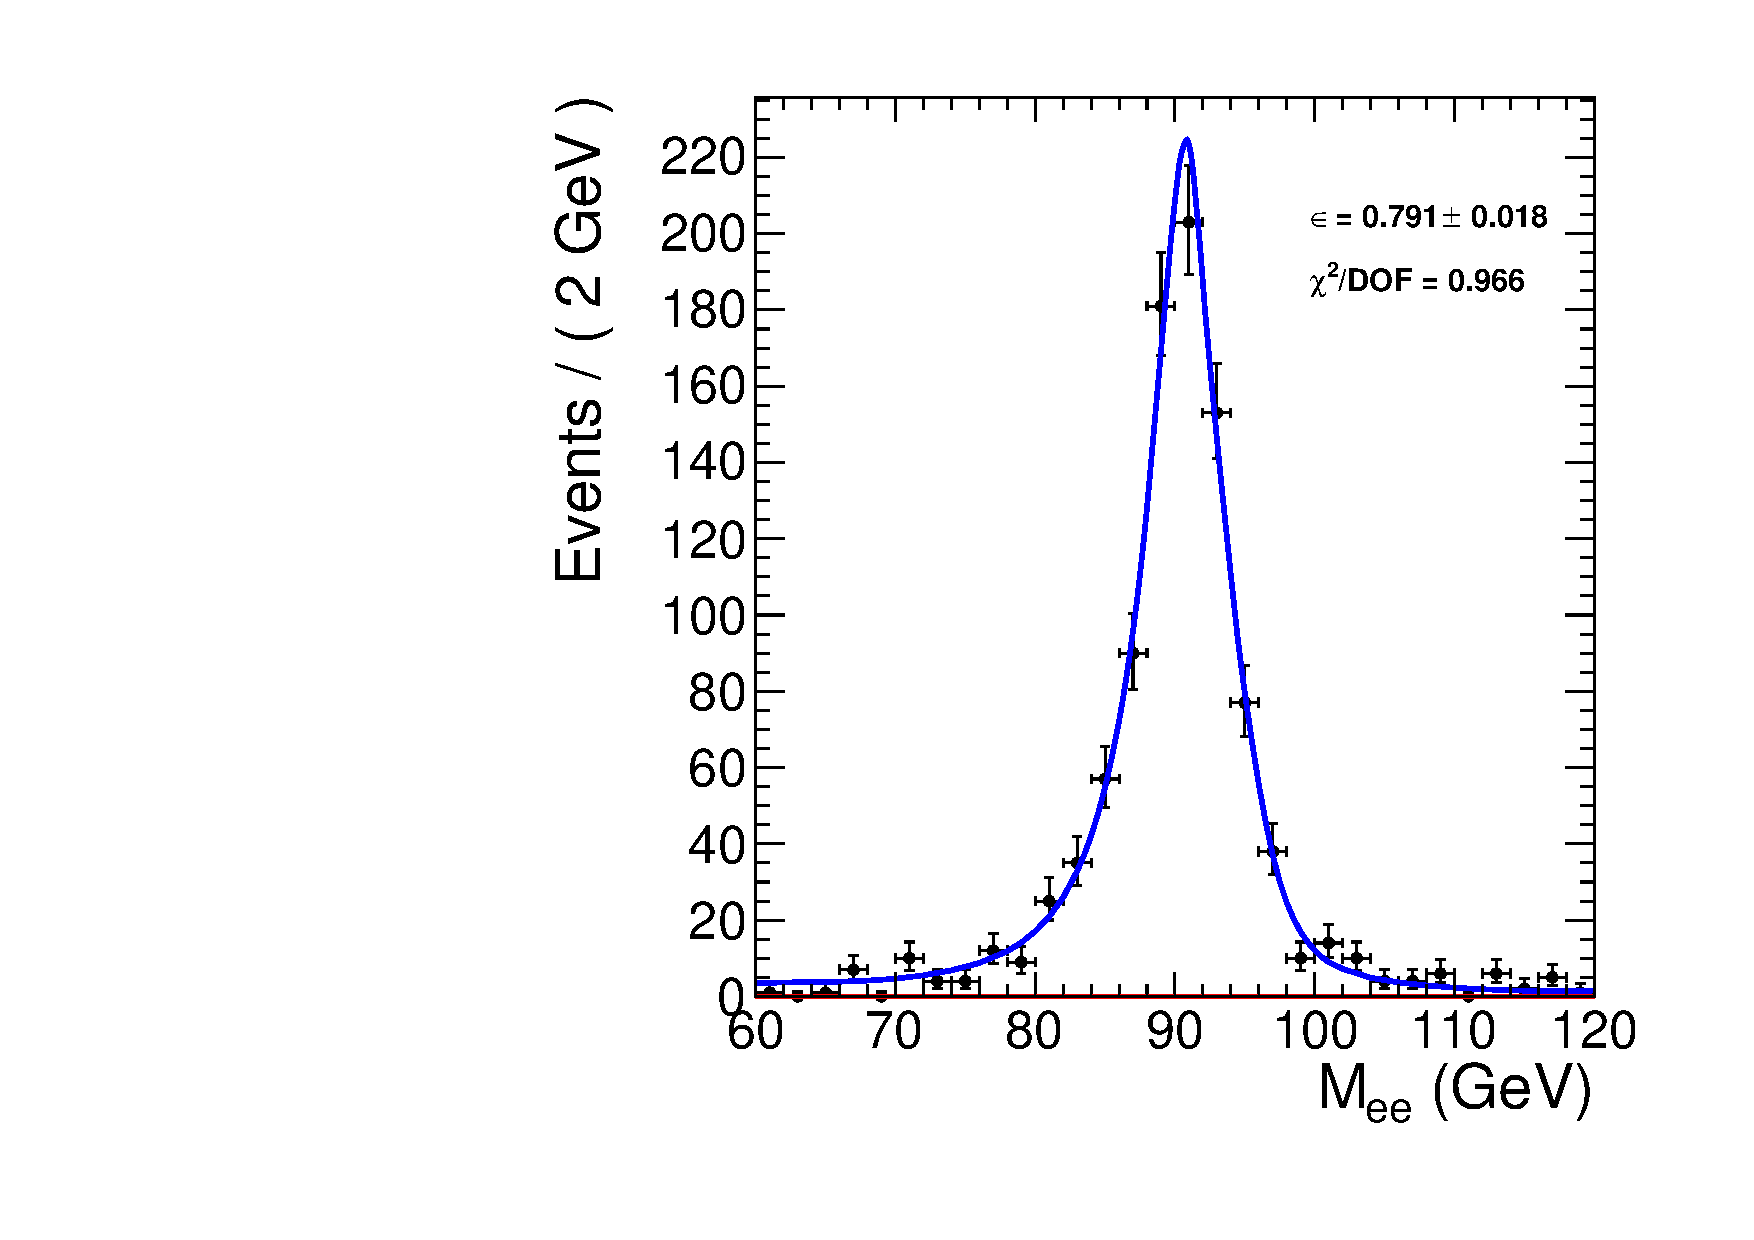
\includegraphics[width=1.0\textwidth]{figs/tpHistos_ID80_eb_pass.pdf}
%  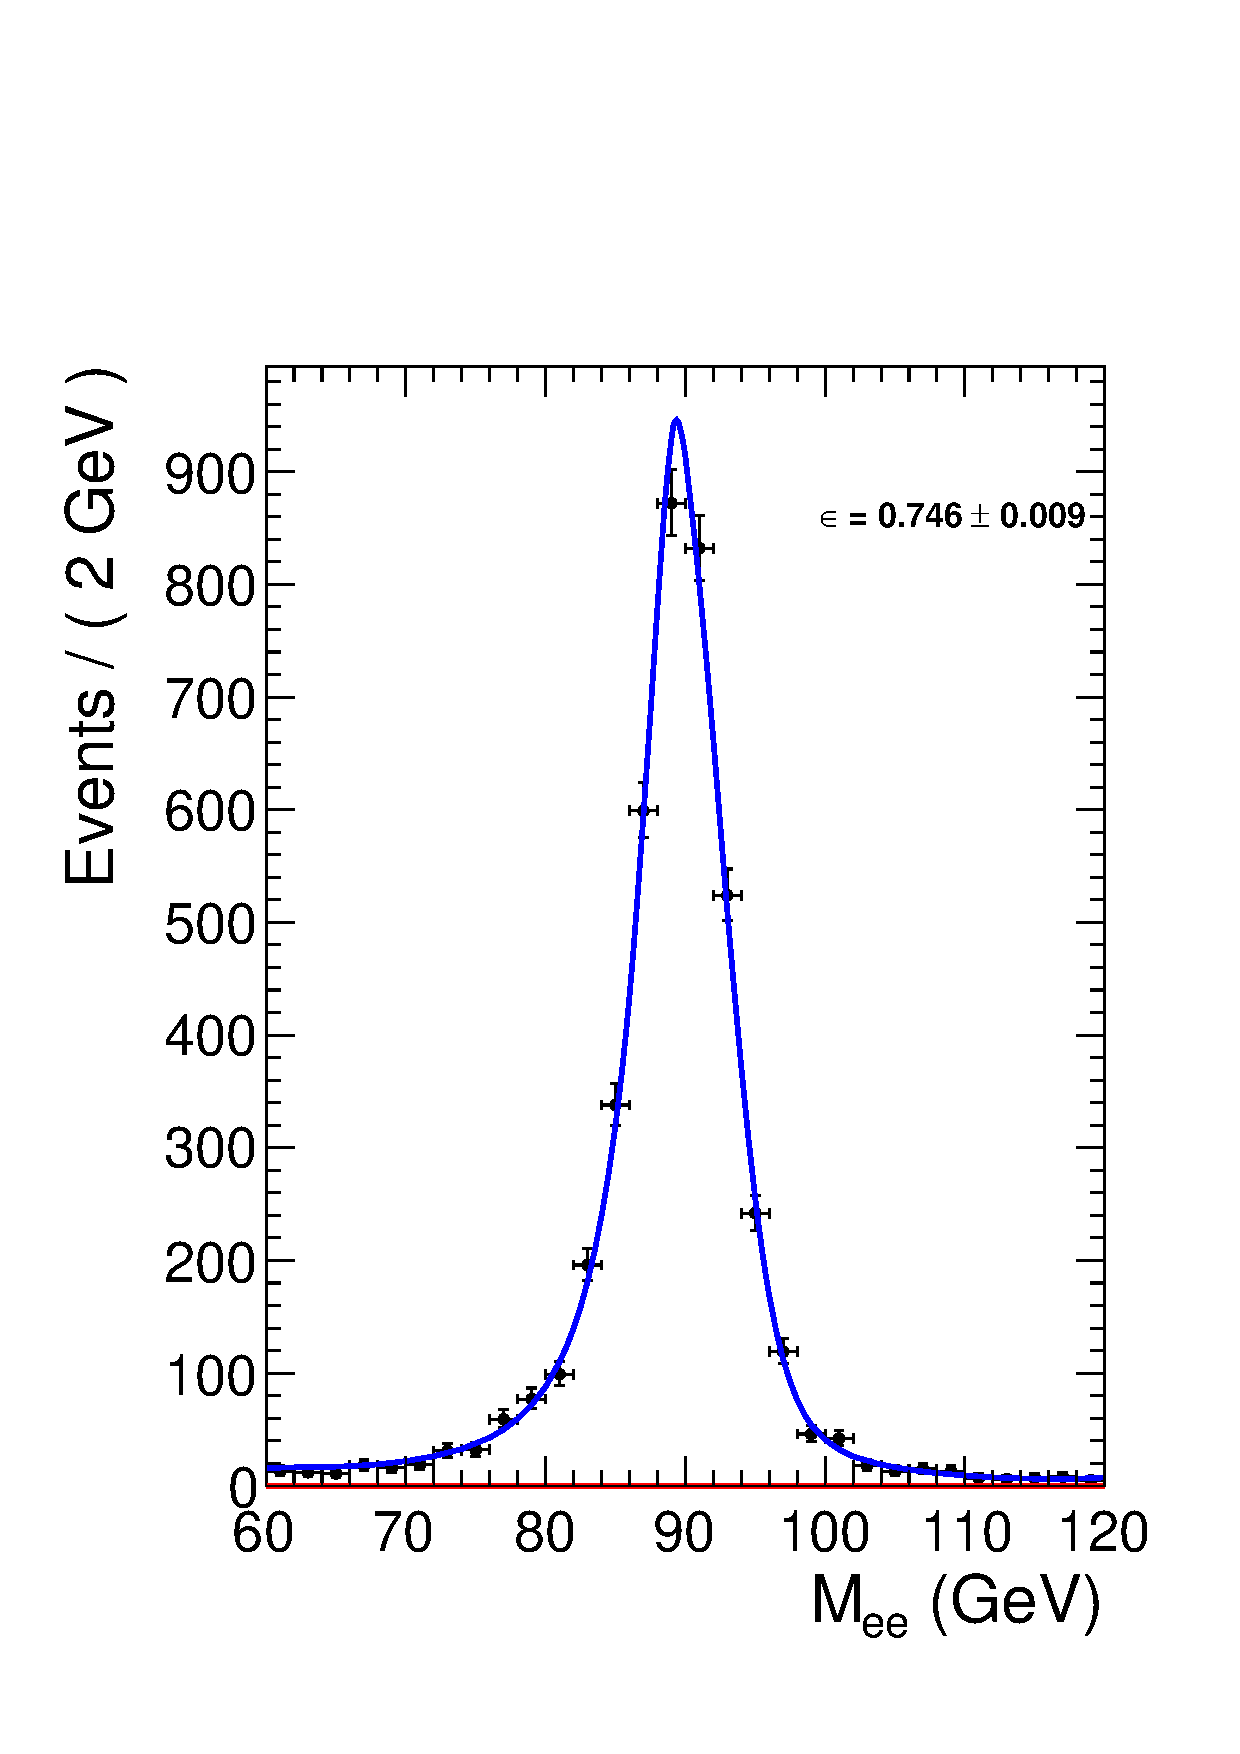
\includegraphics[width=1.0\textwidth]{figs/tpHistos_ID80_ee_pass.pdf}
% \end{minipage}
% \begin{minipage}[WP80]{0.32\textwidth}
%  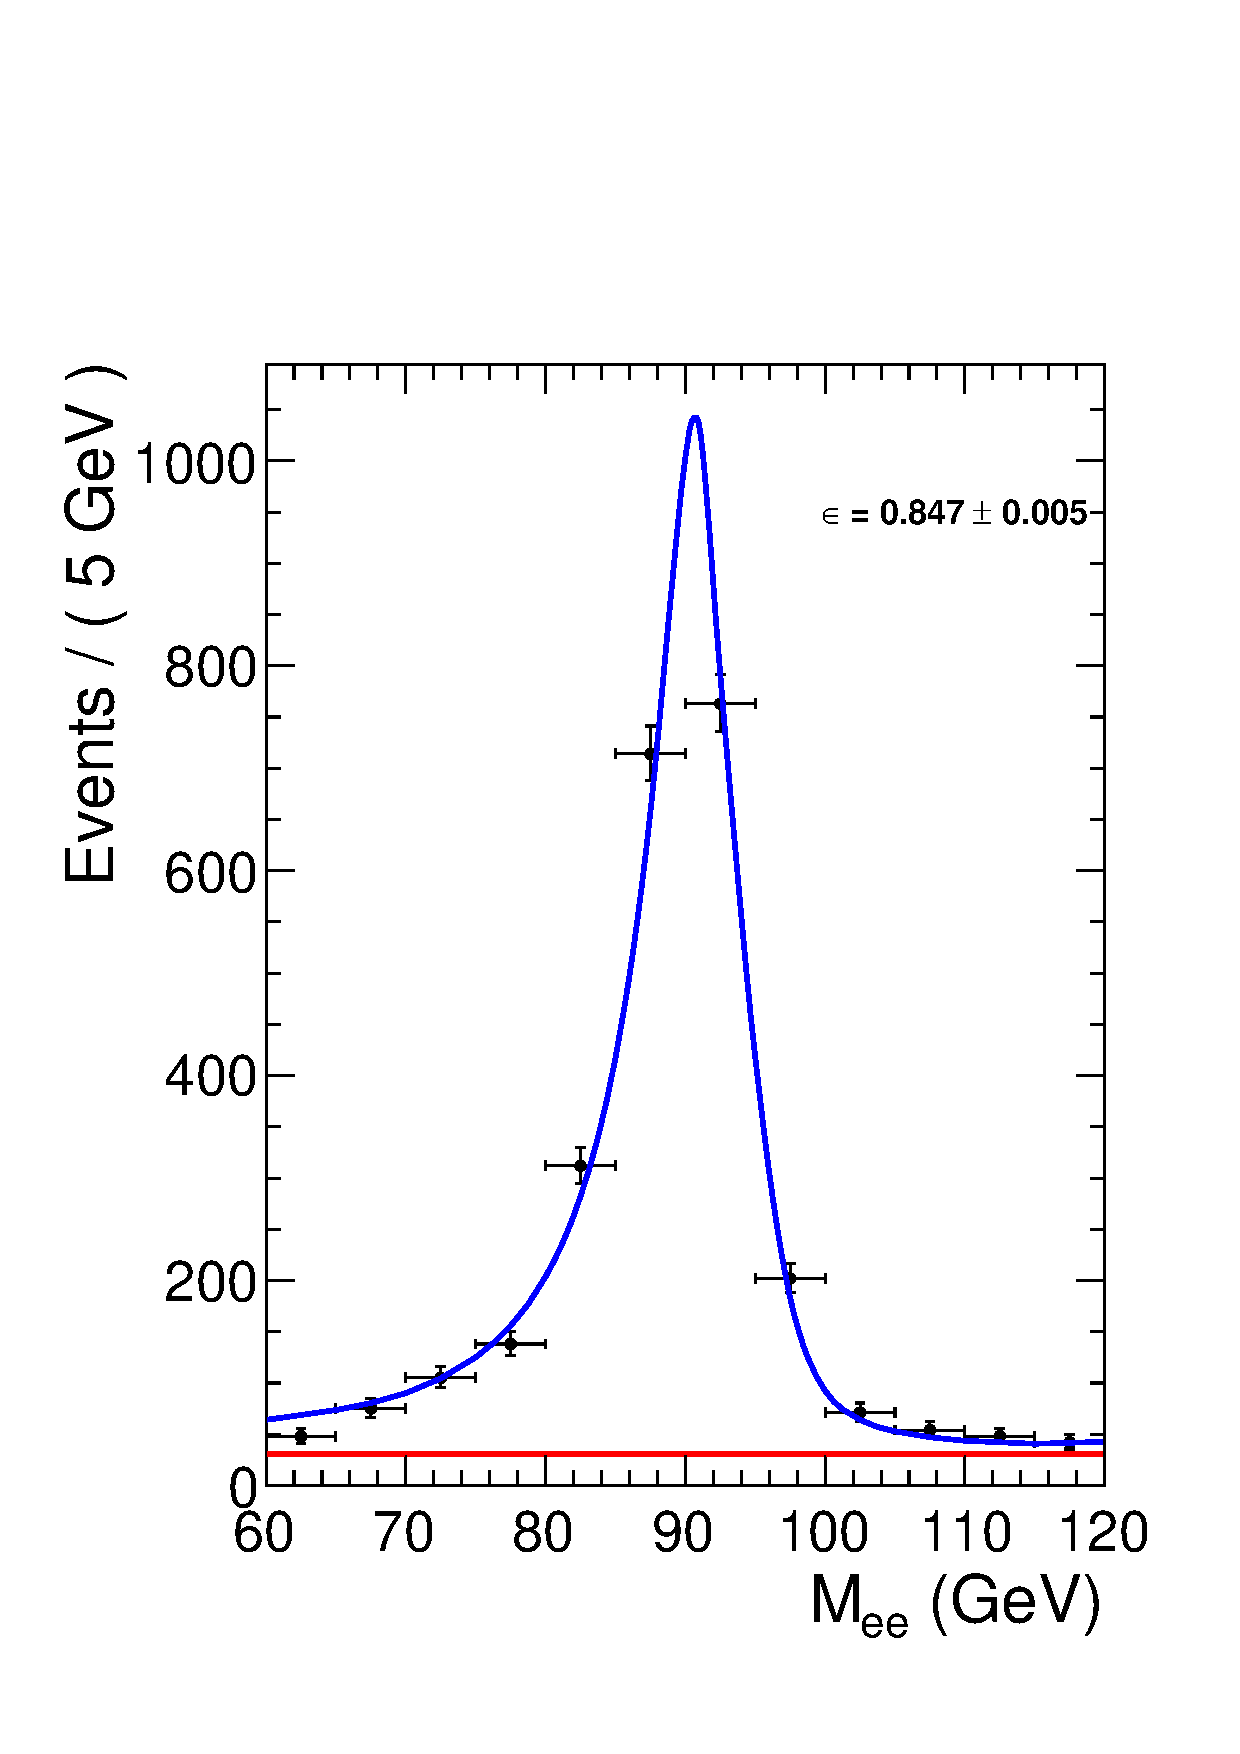
\includegraphics[width=1.0\textwidth]{figs/tpHistos_ID80_eb_fail.pdf}
%  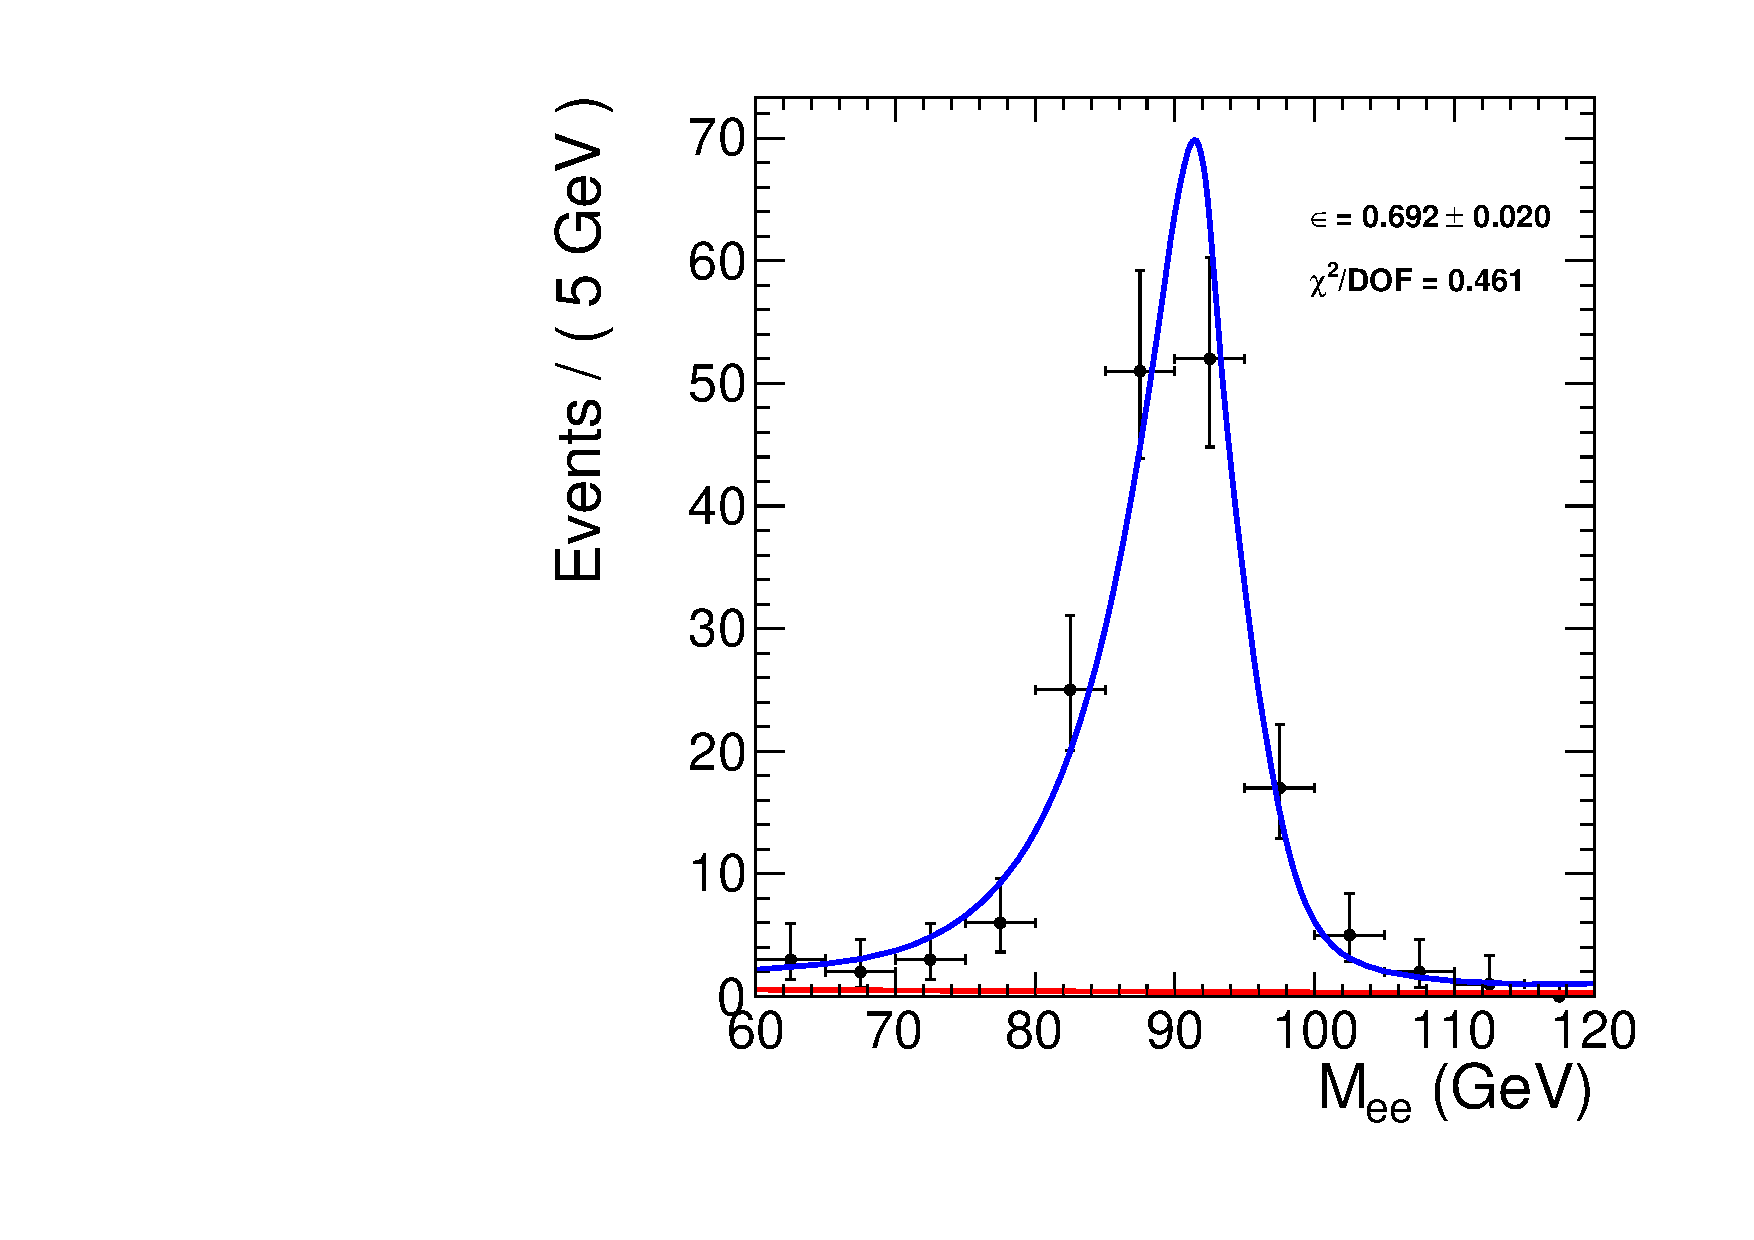
\includegraphics[width=1.0\textwidth]{figs/tpHistos_ID80_ee_fail.pdf}
% \end{minipage}
%% \begin{minipage}[W80toTrigger]{0.32\textwidth}
%%  \includegraphics[width=1.0\textwidth]{figs/TNPe_fake.png}
%%  \includegraphics[width=1.0\textwidth]{figs/TNPe_fake.png}
%% \end{minipage}
% \end{center}
%\caption{Extraction of \TNP efficiencies in the data from fits
%to the dielectron mass distributions for passing (upper row) and failing (lower row) probes:
%GSF-electron $\to$ tight selection for ECAL Barrel (left column) and ECAL Endcaps (right column). 
%The red line represents the background estimation.
%\label{fig:e-TNP}}
%\end{figure}
%Examples of \TNP fits on the data are given in Fig.~\ref{fig:e-TNP}
%for illustration.
%% can't cite an AN
%% All the details of the \TNP fits can be found in~\cite{CMS_AN_2010-323}.


%In addition to efficiencies, we report data/MC efficiency
%ratios $\rhoeff$, also called data/MC correction factors:
%\begin{equation}
%  \rho_{\textrm{eff-X}} = \frac{\EPS{TNP-X}(\textrm{data})}{\EPS{TNP-X}(\textrm{MC})}  \ \ \ 
%\textrm{and} \ \ \ \EPS{X} = \EPS{MC-X} \times \rho_{\textrm{eff-X}} ,
%\end{equation}
%where $\EPS{X}$ is the final electron efficiency
%and $\EPS{MC-X}$, the ``true''
%MC efficiency, for selection $X$ (reco, tight selection, HLT or overall).

The \TNP event selection efficiencies in the simulation 
are determined from large samples of signal events with no
background added.

%The main reason for considering data/MC correction factors rather
%than absolute efficiencies is that some biases cancel in the ratio.
%One bias that affects the $W$ analysis comes from the fact that,
%due limited statistics, we consider only two bins
%in pseudorapidity (EB and EE). In each bin efficiencies are weighted
%by the pseudorapidity distribution of electrons from Z decays,
%which is different from that of electrons from W$^+$ or W$^-$ decays.
%Hence, any $\eta$ dependence of the efficiency within the bin induces
%a bias, which is expected to cancel in the ratio (assuming that
%the dependence is roughly reproduced in the simulation).

The \TNP efficiencies are measured for the EB and EE electrons separately.
Tag-and-probe efficiencies are also determined separately by charge, 
to be used in the measurements of the W$^+$ and W$^-$ cross sections and their ratio.
%For this selection, only the charge of the probe is considered except for the
%determination of the reconstruction efficiency, where the probe (which is an
%ECAL cluster) is assigned the charge opposite to that of the tag.
%Tag-and-probe electron efficiencies, for the data and the Monte Carlo 
%simulation, and efficiency correction factors, are summarized in 
%Table~\ref{tab:e-eff-summary}. 
Inclusive efficiencies and correction factors are summarized in 
Table~\ref{tab:e-eff-summary}. The \TNP measurements of the efficiencies 
on the right-hand side of Eq.~(\ref{eq:e-eff})
are denoted as $\EPSTNPREC$, $\EPS{\tnp-tight}$, and $\EPSTNPTRG$.

%--------------------------------------------------
\begin{table}[htbp] %
\begin{center}
\caption[.]{\label{tab:e-eff-summary}
Tag-and-probe efficiencies in data and simulation, and the correction factors
used in the electron channels for the barrel (EB) and endcaps (EE). The combined statistical and systematic 
uncertainties are quoted. }
\begin{tabular}{|l|c|c|c|}
\hline
Efficiency & Data & Simulation & Data/simulation ($\rhoeff$) \\
\hline
\hline
\multicolumn{4}{|c|}{EB} \\
\hline
 \EPS{\tnp-rec}      & \WPWIEBEFFRECO  & \WPWIEBMCRECO & \WPWIEBRRECO \\
 \EPS{\tnp-tight}    & \WPWIEBEFFID    & \WPWIEBMCID   & \WPWIEBRID   \\
 \EPS{\tnp-trg}      & \WPWIEBEFFHLT   & \WPWIEBMCHLT  & \WPWIEBRHLT  \\
\hline
 \EPS{\tnp-all}  & \WPWIEBEFF  & \WPWIEBMC & \WPWIEBR \\
\hline
\hline
\multicolumn{4}{|c|}{EE} \\
\hline
 \EPS{\tnp-rec}       & \WPWIEEEFFRECO  & \WPWIEEMCRECO & \WPWIEERRECO \\
 \EPS{\tnp-tight}    & \WPWIEEEFFID    & \WPWIEEMCID   & \WPWIEERID   \\
 \EPS{\tnp-trg} & \WPWIEEEFFHLT   & \WPWIEEMCHLT  & \WPWIEERHLT  \\
\hline
 \EPS{\tnp-all}  & \WPWIEEEFF  & \WPWIEEMC & \WPWIEER \\
\hline
\end{tabular}
\end{center}
\end{table}


\par
Event selection efficiencies are measured with respect to the W events
within the ECAL acceptance.
Simulation efficiencies estimated from {\sc POWHEG} $\Wo$ samples 
are shown in Table~\ref{tab:el-Weff}.
These are efficiencies at the event level,
e.g.: they include efficiency loss due to the second electron veto.  
Given the acceptances listed in Table~\ref{tab:WZlaccgen} and the \TNP 
efficiencies listed in Table~\ref{tab:e-eff-summary},
the overall efficiency correction factors for electrons from $\Wo$ decays are computed.
The overall $\Wo$ signal efficiencies, obtained as products of simulation efficiencies
with data/simulation correction factors, are listed in Table~\ref{tab:el-Weff}.
%These efficiencies are relative to $\Wo$ events with the electron within the acceptance,
%as described above. 
%Theoretical uncertainties on the efficiencies related to the PDF uncertainties and 
%the PDF choice are negligible.
\begin{table}[ht] %
  \begin{center}
  \caption{ Simulation efficiencies and the final corrected selection efficiencies for the 
$\Wp$, $\Wm$, and their average, in the $\Wen$ analysis. The quoted uncertainties are 
statistical for $\effmc$ and include both statistical and systematic uncertainties 
for the corrected efficiencies $\effmc \times \rhoeff$.
  \label{tab:el-Weff}}
  \begin{tabular}{|l|c|c|}
    \hline
     & $\effmc$  &  $\effmc \times \rhoeff$ \\
    \hline\hline
 $\Wpen$   & \WEPEFFMC  & \WEPEFF \\
 $\Wmen$   & \WEMEFFMC  & \WEMEFF \\
 $\Wen$  & \WEIEFFMC  & \WEIEFF \\
    \hline
    \end{tabular}
  \end{center}
\end{table}

The efficiencies and the data/simulation ratios are also estimated in bins of the electron 
$\Et$ and $\eta$ in order to examine in detail the detector performance and take into 
account the differences in the W and Z kinematic distributions. 
The data/simulation ratios for reconstruction, selection, and trigger are shown 
in Fig.~\ref{fig:e-TnPratios} as functions of the electron $\Et$ and $\eta$.

The reconstruction data/simulation ratios appear to be uniform with respect to $\Et$ and $\eta$, so
a smaller number of bins is sufficient for the determination of their values.
%Based on this fact our choice was to quote as reconstruction 
%efficiency the estimation in two $\eta$ bins only (in ECAL Barrel and ECAL Endcaps).
The data/simulation ratios for the selection and trigger efficiencies show a dependence 
that is estimated using ten $\eta$ bins and six $\Et$ bins. Data/simulation ratios are estimated for 
both electron charges as well. 

The binned ratios and simulation efficiencies are transferred into the W analysis by properly weighting 
their product in each ($\Et$, $\eta$) bin by the relative ECAL cluster abundance
estimated from {\sc POWHEG} simulations. The corrected efficiencies are compared with the 
two-bin case in which the efficiencies are estimated in two bins of $\eta$ (EB and EE). 
The multibin corrected efficiencies are found to be consistent with the  two-bin 
corrected efficiencies within the assigned uncertainties. 
% In order to be sure that no hidden systematic uncertainty is missed,  half of the 
% maximum difference between the multibin and two-bin corrected efficiencies 
% is propagated as an additional systematic uncertainty on the two-bin efficiencies used to estimate the cross 
% sections. The additional relative uncertainty is at the level of 0.6$\%$.  


\begin{figure}[htbp]
\begin{center}
% \begin{minipage}[Reconstruction]{0.64\textwidth}
  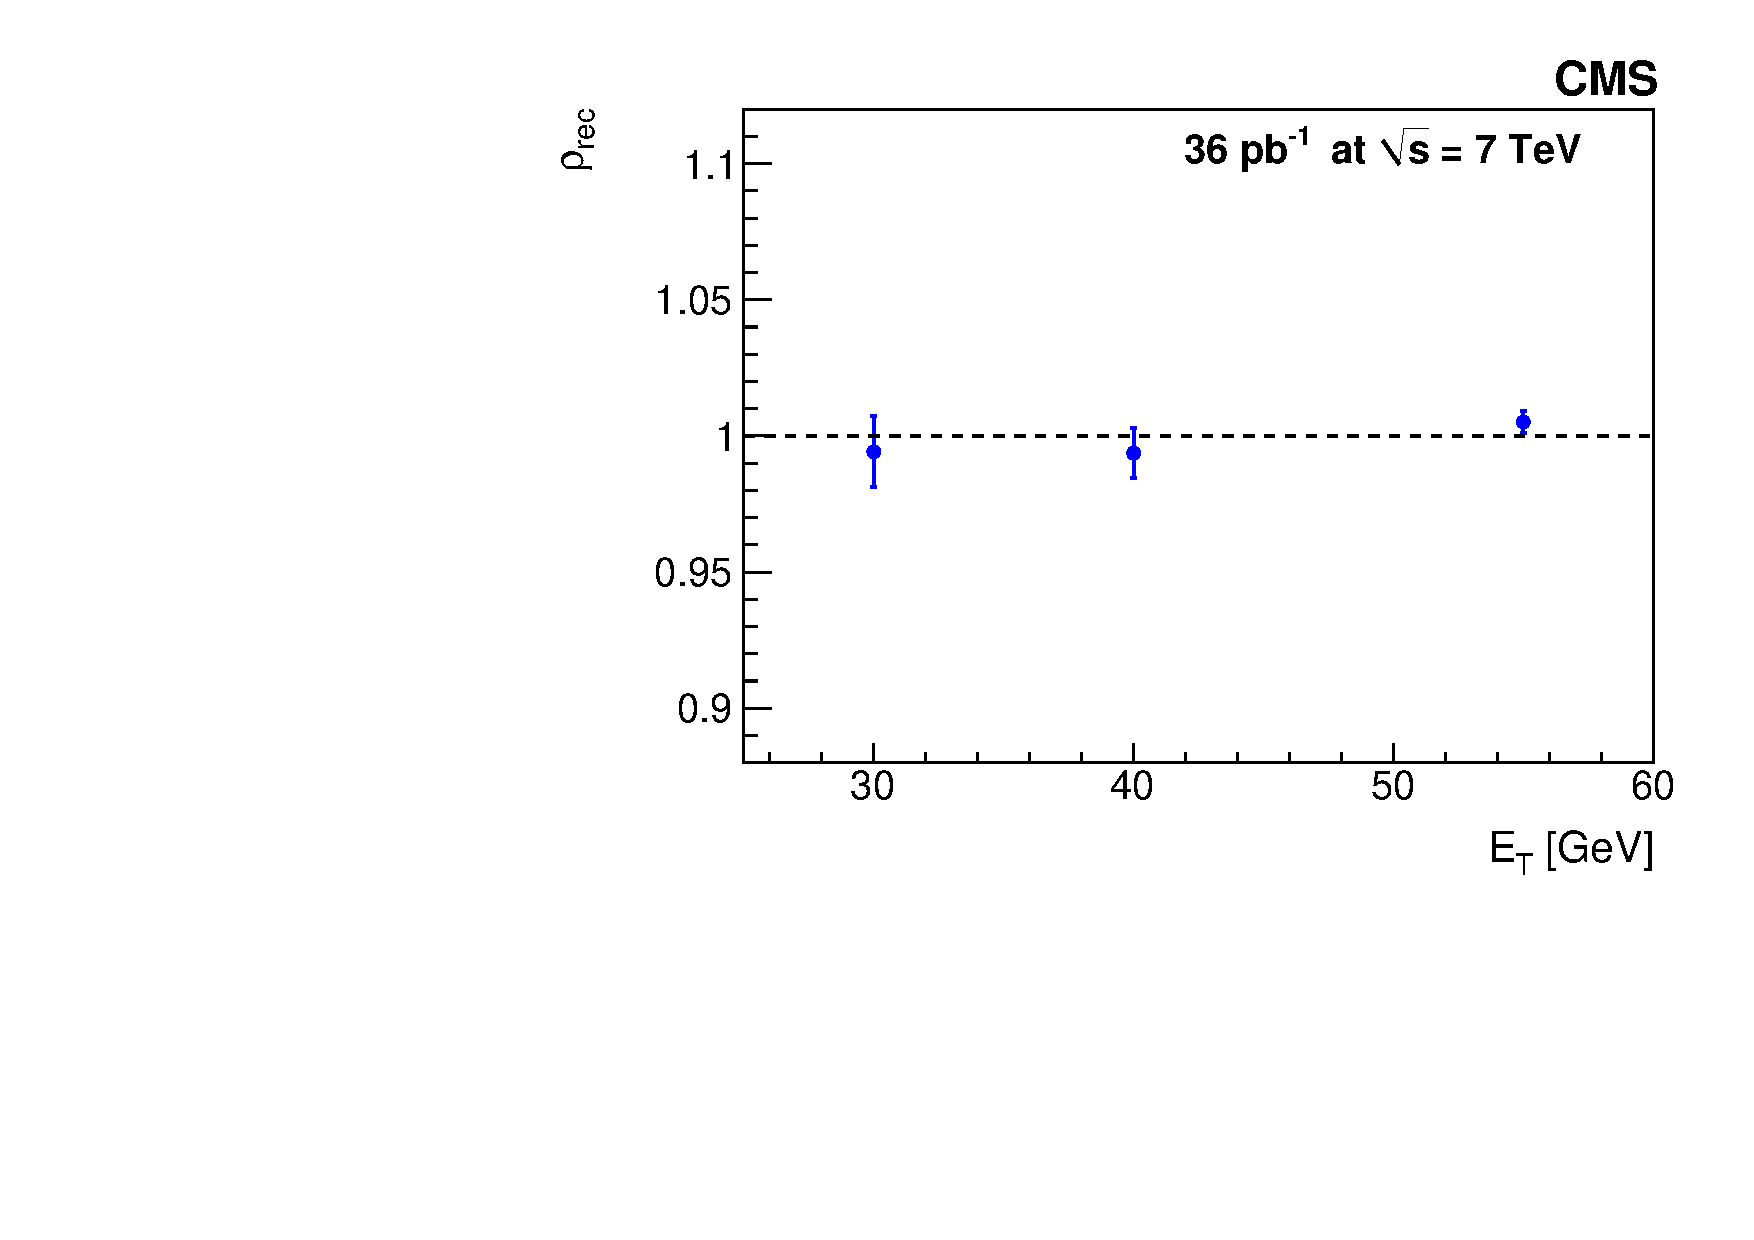
\includegraphics[width=0.48\textwidth]{figs/recoeff_scalept.pdf}
  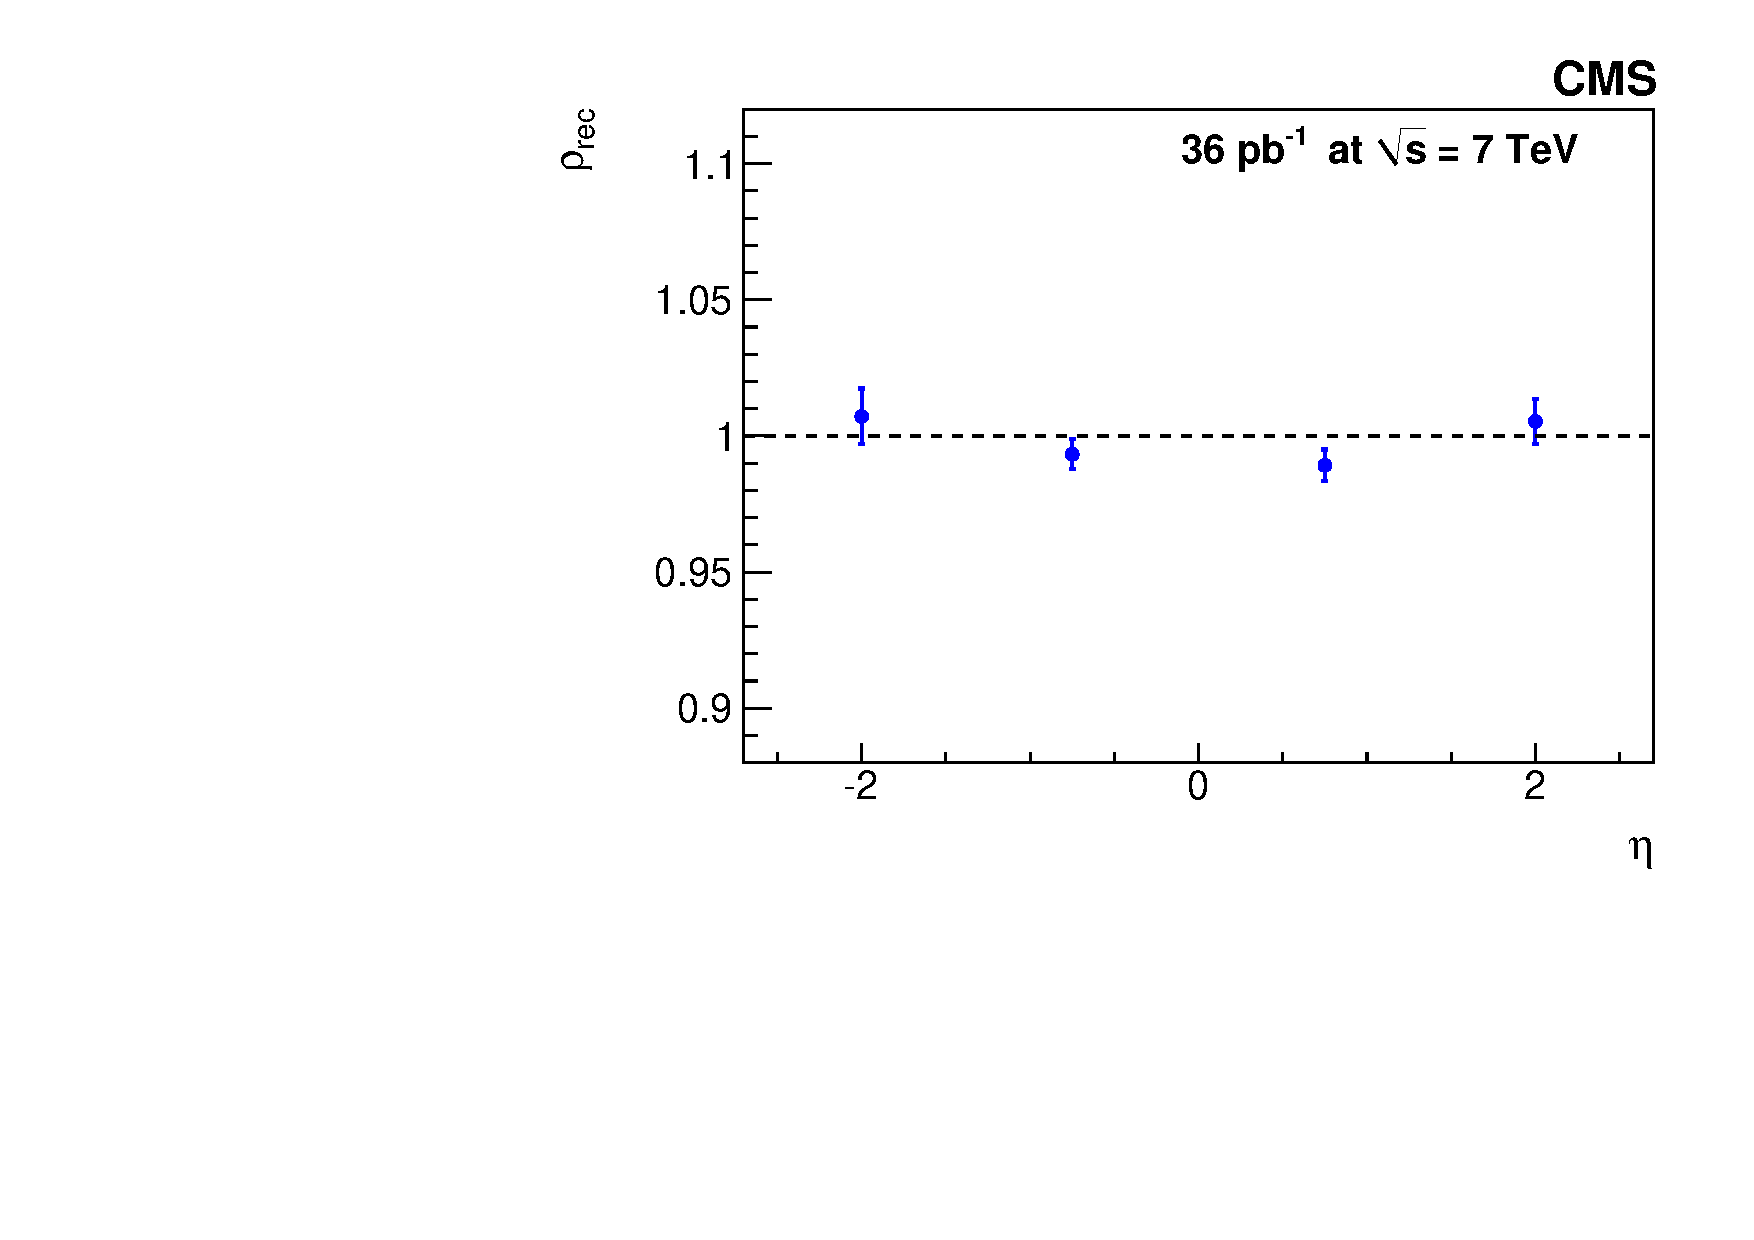
\includegraphics[width=0.48\textwidth]{figs/recoeff_scaleeta.pdf}
% \end{minipage}
% \begin{minipage}[WP80]{0.64\textwidth}
  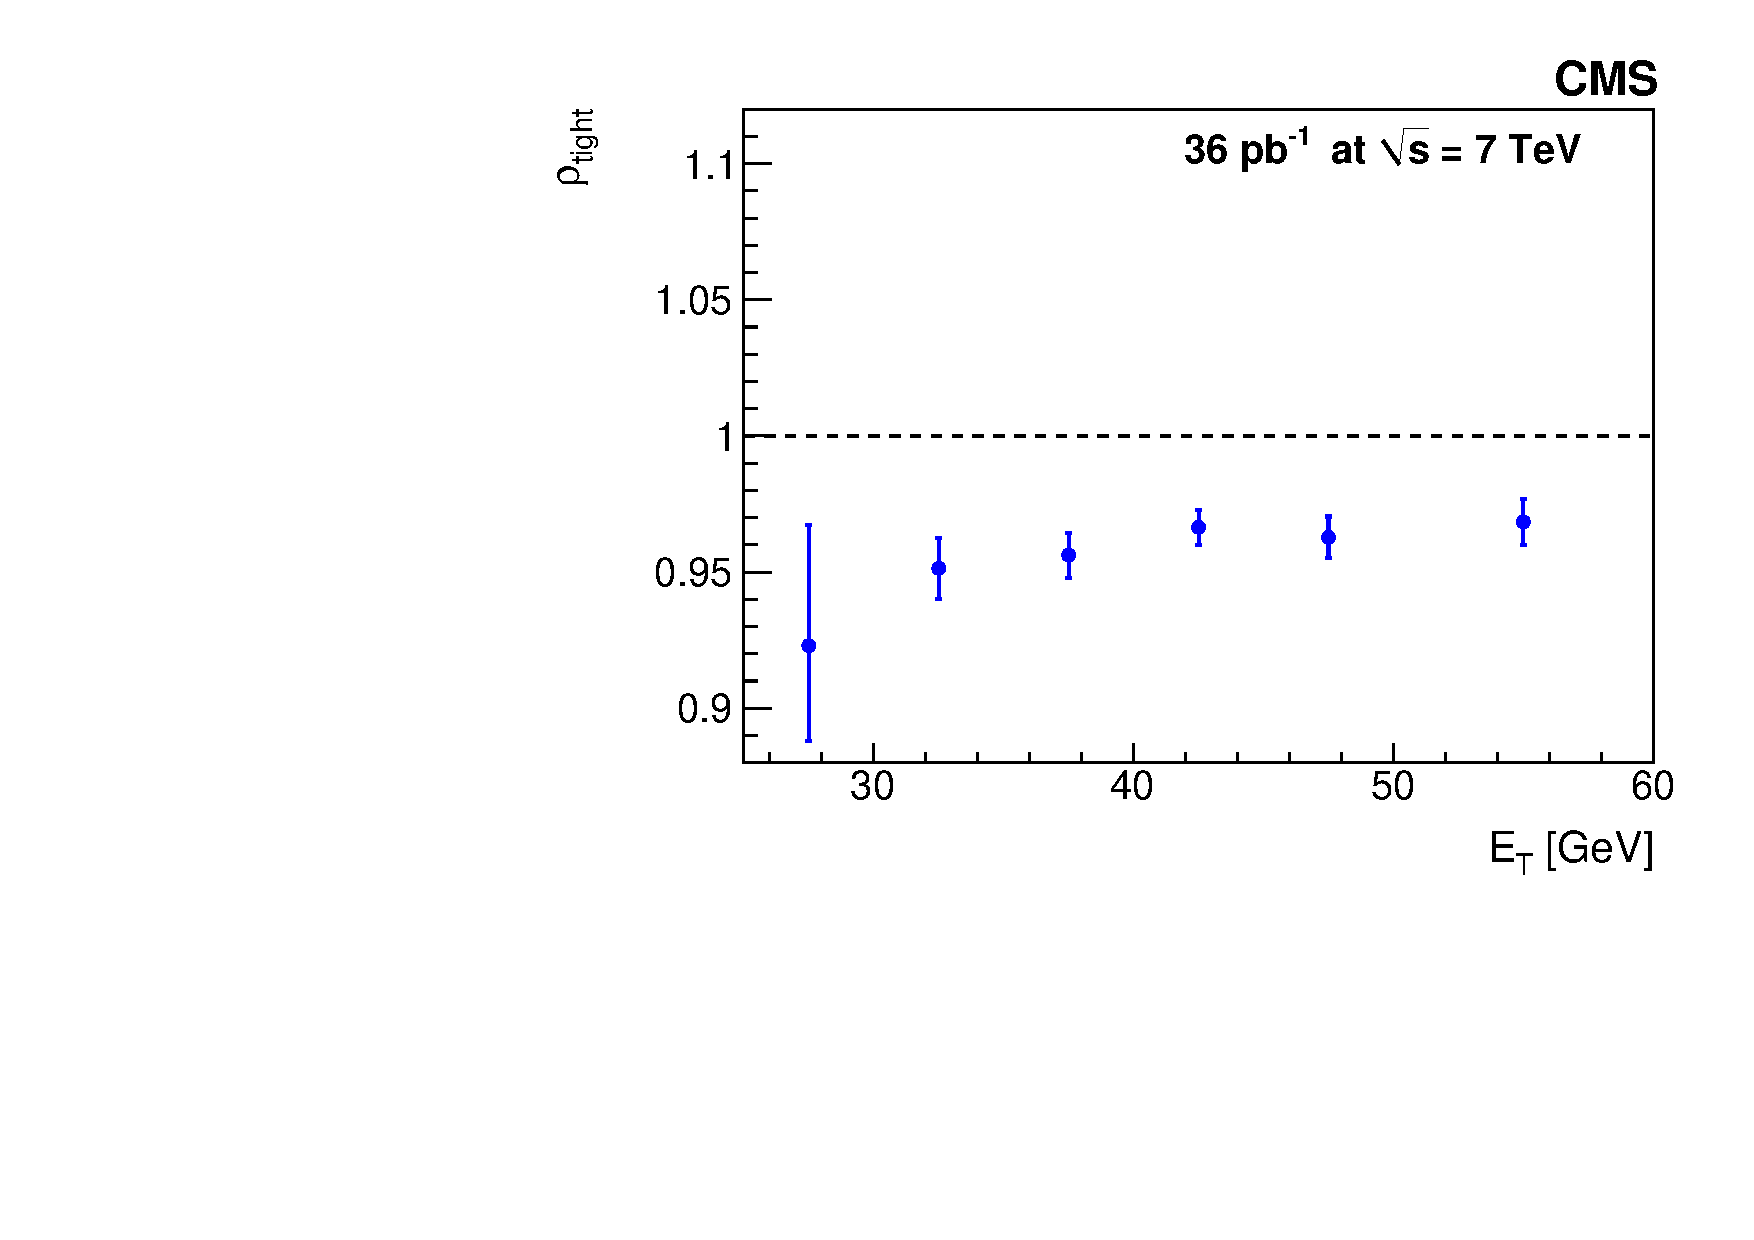
\includegraphics[width=0.48\textwidth]{figs/eleideff_scalept.pdf}
  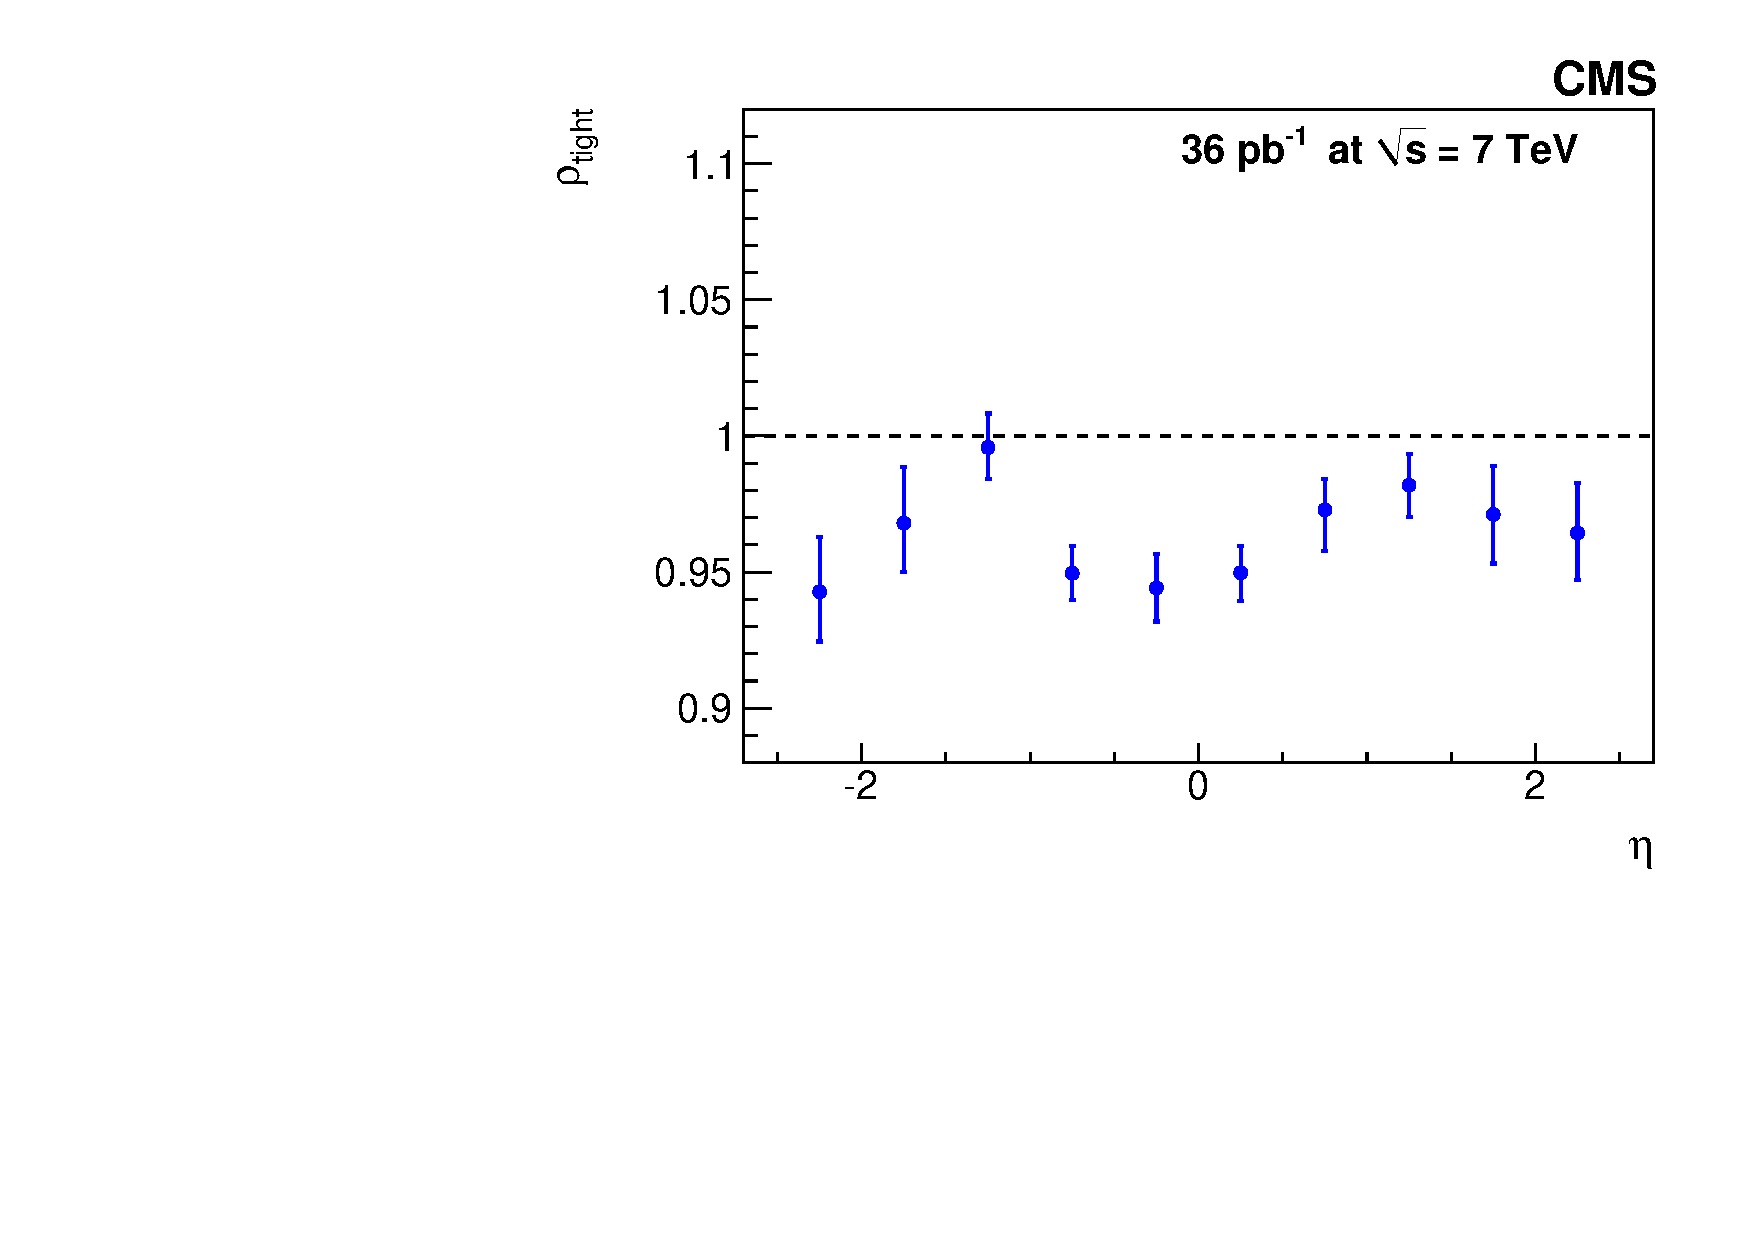
\includegraphics[width=0.48\textwidth]{figs/eleideff_scaleeta.pdf}
% \end{minipage}
% \begin{minipage}[W80toTrigger]{0.64\textwidth}
  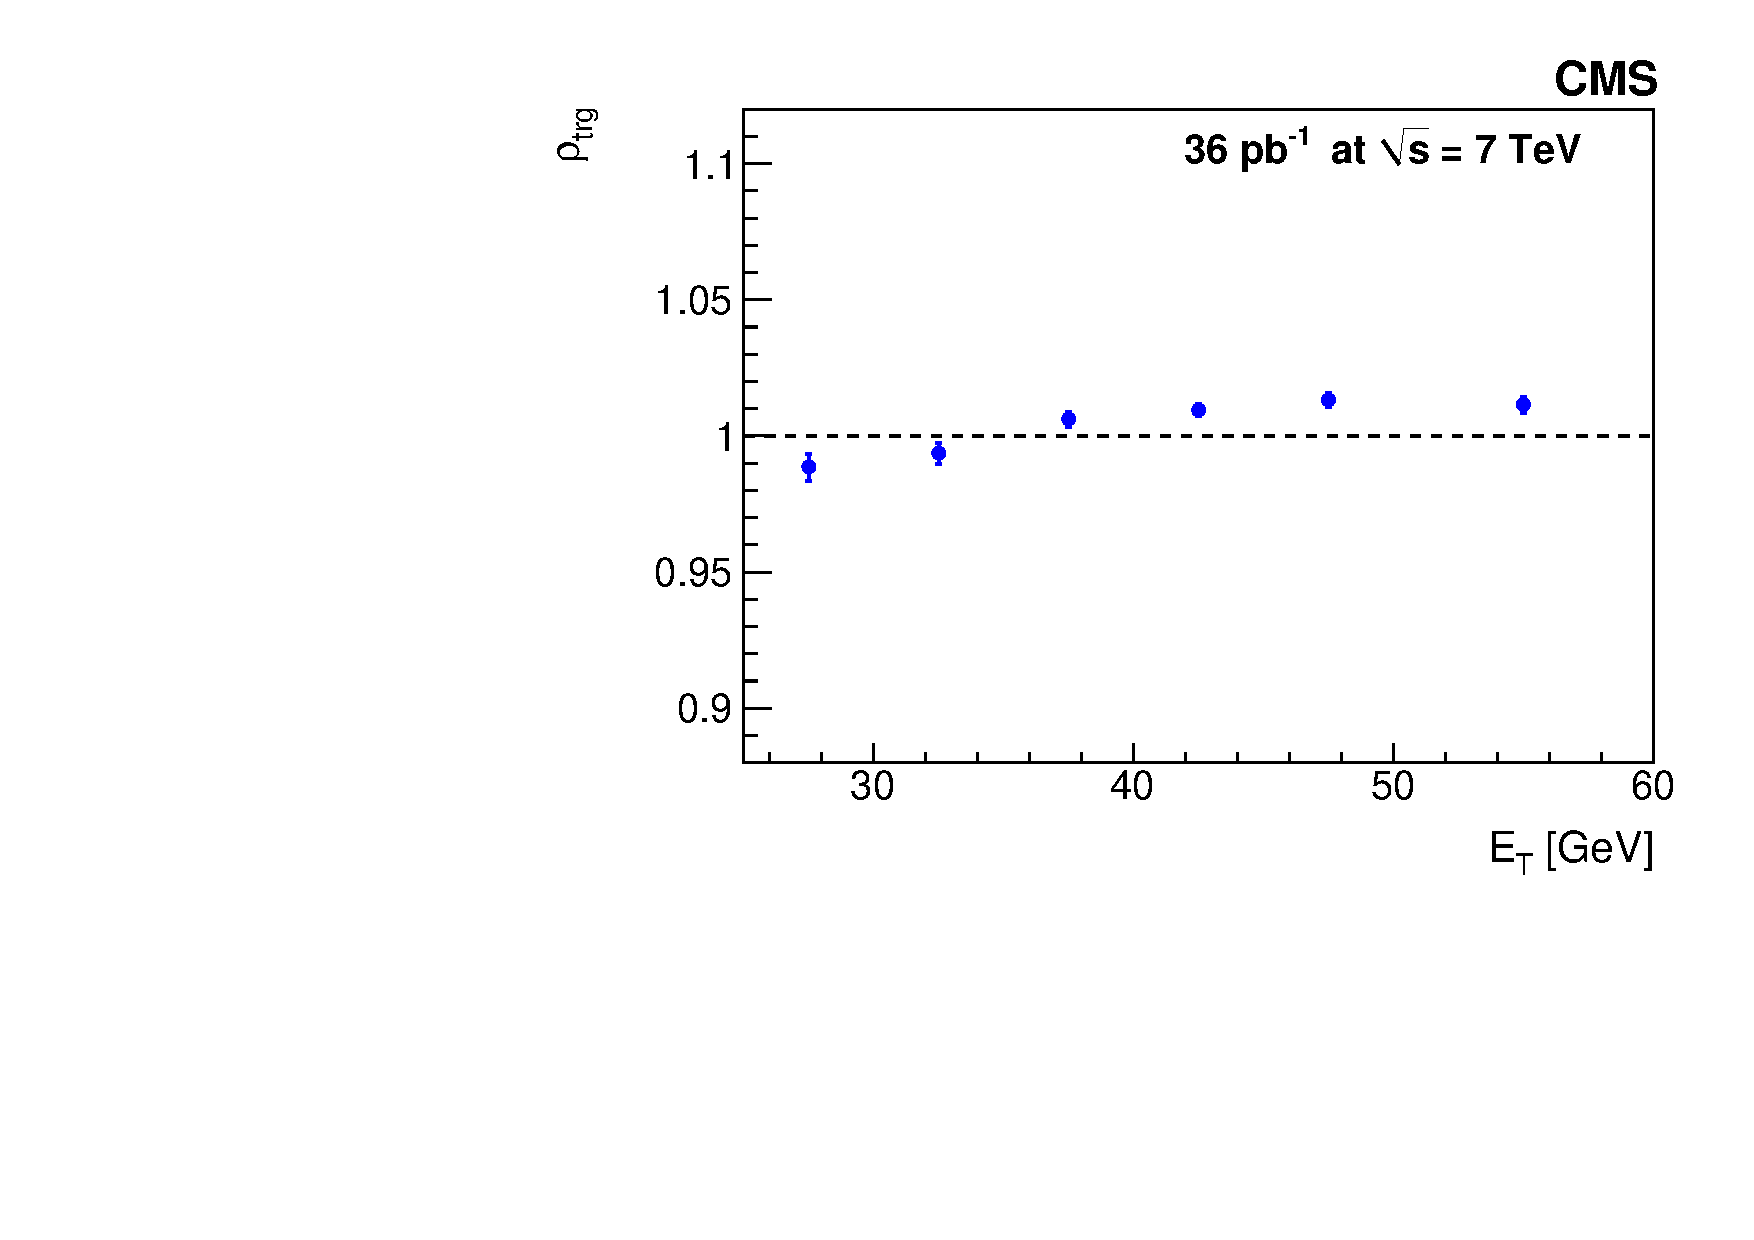
\includegraphics[width=0.48\textwidth]{figs/trigeff_scalept.pdf}
  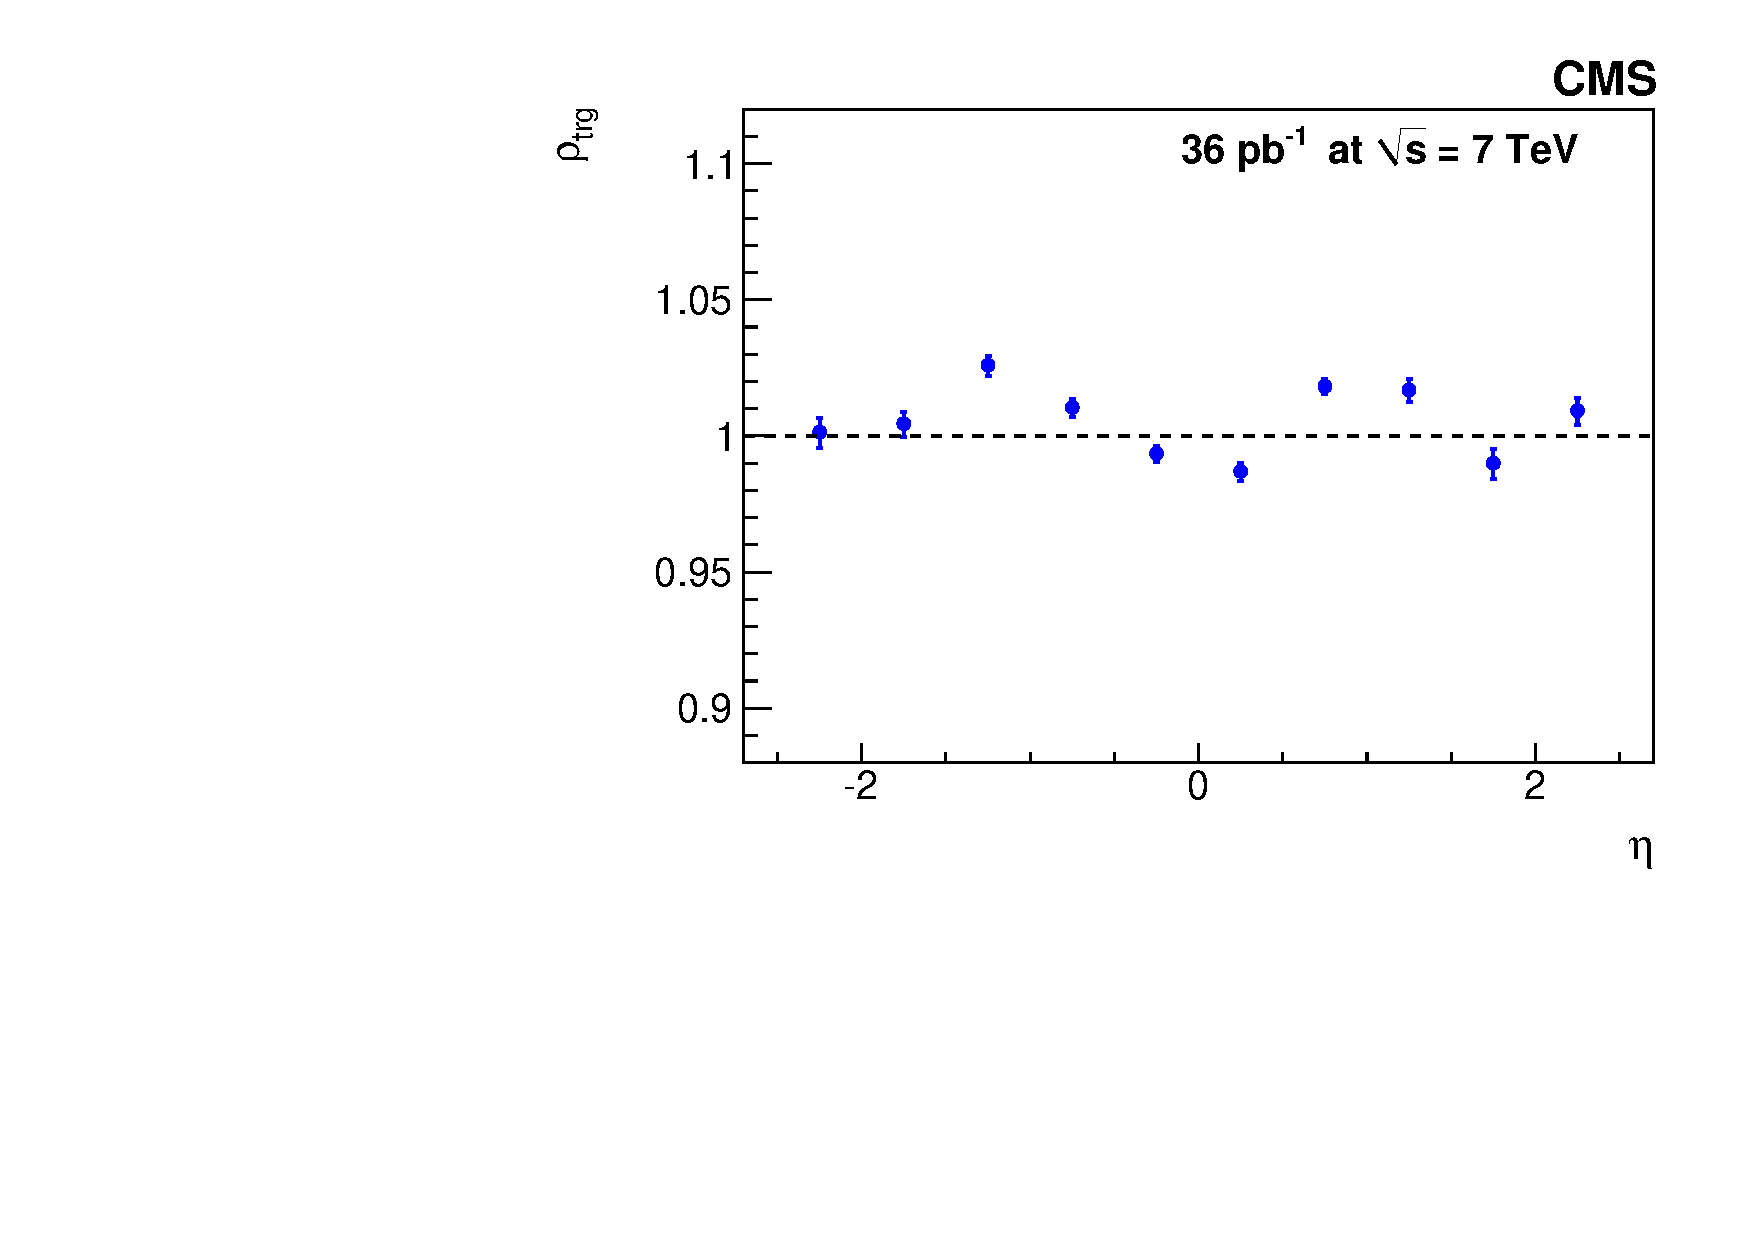
\includegraphics[width=0.48\textwidth]{figs/trigeff_scaleeta.pdf}
% \end{minipage}
 \end{center}
\caption{Data/simulation \TNP ratios versus electron $\Et$ (left column) and $\eta$ (right column).
The ratios are presented for the reconstruction ($\rho_\mathrm{rec}$, top row), selection 
($\rho_\mathrm{tight}$, middle row), and trigger ($\rho_\mathrm{trg}$, bottom row) efficiencies.
Points with error bars represent the ratio measured in data; dashed lines correspond to a constant ratio of one.
\label{fig:e-TnPratios}}
\end{figure}


The $\Zo$ selection efficiencies for data and simulation are obtained based
on the \TNP efficiencies
listed in Table~\ref{tab:e-eff-summary}  and
the event acceptances given in Table~\ref{tab:WZlaccgen}.
The $\Zo$ efficiencies are first determined after
reconstruction and identification (as products of
single-electron efficiencies).
The event trigger efficiency is computed
as the probability that at least one of the two electrons
satisfies the L1+HLT requirement. 
The overall selection efficiency for the $\Zo$ analysis is
the product of the reconstruction, identification, and trigger 
efficiencies. The simulation efficiency obtained from the {\sc POWHEG} $\Zo$ 
samples, together with the final corrected $\Zo$ selection efficiency 
$\effmc \times \rhoeff$, are shown in Table~\ref{tab:el-Zeff}.
These efficiencies are relative to the $\Zo$ events with both electrons within the ECAL acceptance.
%Similarly to the W case, the PDF uncertainties on the corrected $\Zo$ efficiencies 
%were found to be negligible.
\begin{table}[ht] %
  \begin{center}
  \caption{ Simulation efficiency and the final corrected selection efficiency for the ~$\Zee$ analysis.
The quoted uncertainties are statistical for $\effmc$ and include both statistical and 
systematic uncertainties for the corrected efficiency $\effmc \times \rhoeff$.
 \label{tab:el-Zeff}}
  \begin{tabular}{|l|c|c|}
    \hline
     & $\effmc$ & $\effmc \times \rhoeff$ \\
    \hline\hline
    $\Zee$  & \ZEEEFFMC & \ZEEEFF \\
    \hline
    \end{tabular}
  \end{center}
\end{table}


\par
%For later convenience, we define the quantity $A^{\prime}$, which is 
%the overall selection efficiency in the Monte Carlo simulation, as:
%\begin{equation}
%  A^{\prime} = A \times \epsilon
%            = A^{\textrm{ECAL}} \times \EPS{MC} \ .
%\end{equation}




%\subsection{Muon Efficiencies \label{sec:muonEff}}

The muon reconstruction overall selection efficiency 
is determined by the efficiency to find a track in the inner tracker and in the
muon chambers, to pass the isolation requirements, and the probability 
to pass the L1 trigger and HLT.

Tag-and-Probe method is used to determine muon efficiencies for $\Wmn$ cross section determination,
while for $\Zmm$ muon efficiencies are determined simultaneously with the Z yield using a simultaneous
fit technique that is described in Section~\ref{sec:Zmumu}. 
%Tag-and-Probe method uses a clean sample of $\Zmm$ candidates selected from the 36~pb$^{-1}$ available data
%on which about 22000 triggered muon {\em tags} are selected.
%$\Zmm$ events have muon kinematics very similar to those used in the $\Wo$ analysis.
%The possible presence of background processes in the selected event sample has been also taken into account.

%, making use of the 2 million events
%The efficiency ratio 
%$\rho_\mu = {\epsilon_{\mathrm{data}}}/{\epsilon_{\mathrm{MC}}}$ 
%has been calculated in order to be applied to the  
%W cross-section determination. 
The efficiencies have been studied as a function of muon pseudorapidity and transverse momentum, 
to reproduce better the real detector performance. 
The promediated efficiencies are estimated to be
$\epsilon_{\mathrm{data}} = 0.8548 \pm 0.0025\, \mathrm{(stat)} \pm  0.024\, \mathrm{(syst)}$ and
$\epsilon_{\mathrm{MC}} = 0.8989  \pm   0.0004\, \mathrm{(stat)}$ in data and Monte Carlo respectively,
hence a correction factor of $\rho_\mu= 0.9509 \pm  0.0028 \mathrm{(stat)} \pm  0.024\, \mathrm{(syst)}$
has been appled to the data.
The quoted systematic errors take into account the fit parameter uncertainties stemming 
from the correction of the background.

Single-muon efficiencies have also been determined separating in positive or negative charged muons, 
obtaining the following correction factors: $\rho_\mu^+ = 0.957 \pm 0.004\,\mathrm{(stat)} \pm 0.024\,\mathrm{(syst)}$,
$\rho_\mu^- = 0.945 \pm 0.004\,\mathrm{(stat)} \pm 0.024\,\mathrm{(syst)}$.

A small fraction (0.5\%) of muon events is lost because of Level-1 trigger pre-firing
due to the wrong assignment to the muon bunch crossing number, due to imperfect timing. 
Cross sections in muon channels have been corrected by this effect and
the uncertainty on the correction factor has been taken as systematic uncertainty.


